\begin{definition}
    Definiujemy rozkład normalny (uogólniony) jako rozkład o następującej funkcji gęstości prawdopodobieństwa: 

    \[ f_Z(z) =  \frac{1}{\sigma\sqrt{2\pi}}e^{-((z - \mu)/\sigma)^2/2} \]
\end{definition}

\begin{definition}
    Rozkład normalny o parametrach \(\mu\) i \(\sigma^2\) oznaczamy jako \(N(\mu , \sigma^2 )\).
\end{definition}

\begin{definition}
    Standardowy rozkład Normalny to rozkład normalny o parametrach \( \mu = 0\) i \( \sigma^2 = 1\); oznaczamy go (bez większego szoku) jako \(N(0, 1)\).
\end{definition}

\begin{definition}
    Dystrybuantę standardowego rozkładu normalnego oznaczamy jako \( \Phi \).
\end{definition}

Funkcja gęstości prawdopodobieństwa standardowego rozkładu normalnego wygląda jak \sout{dzban} dzwon.

\begin{center}
    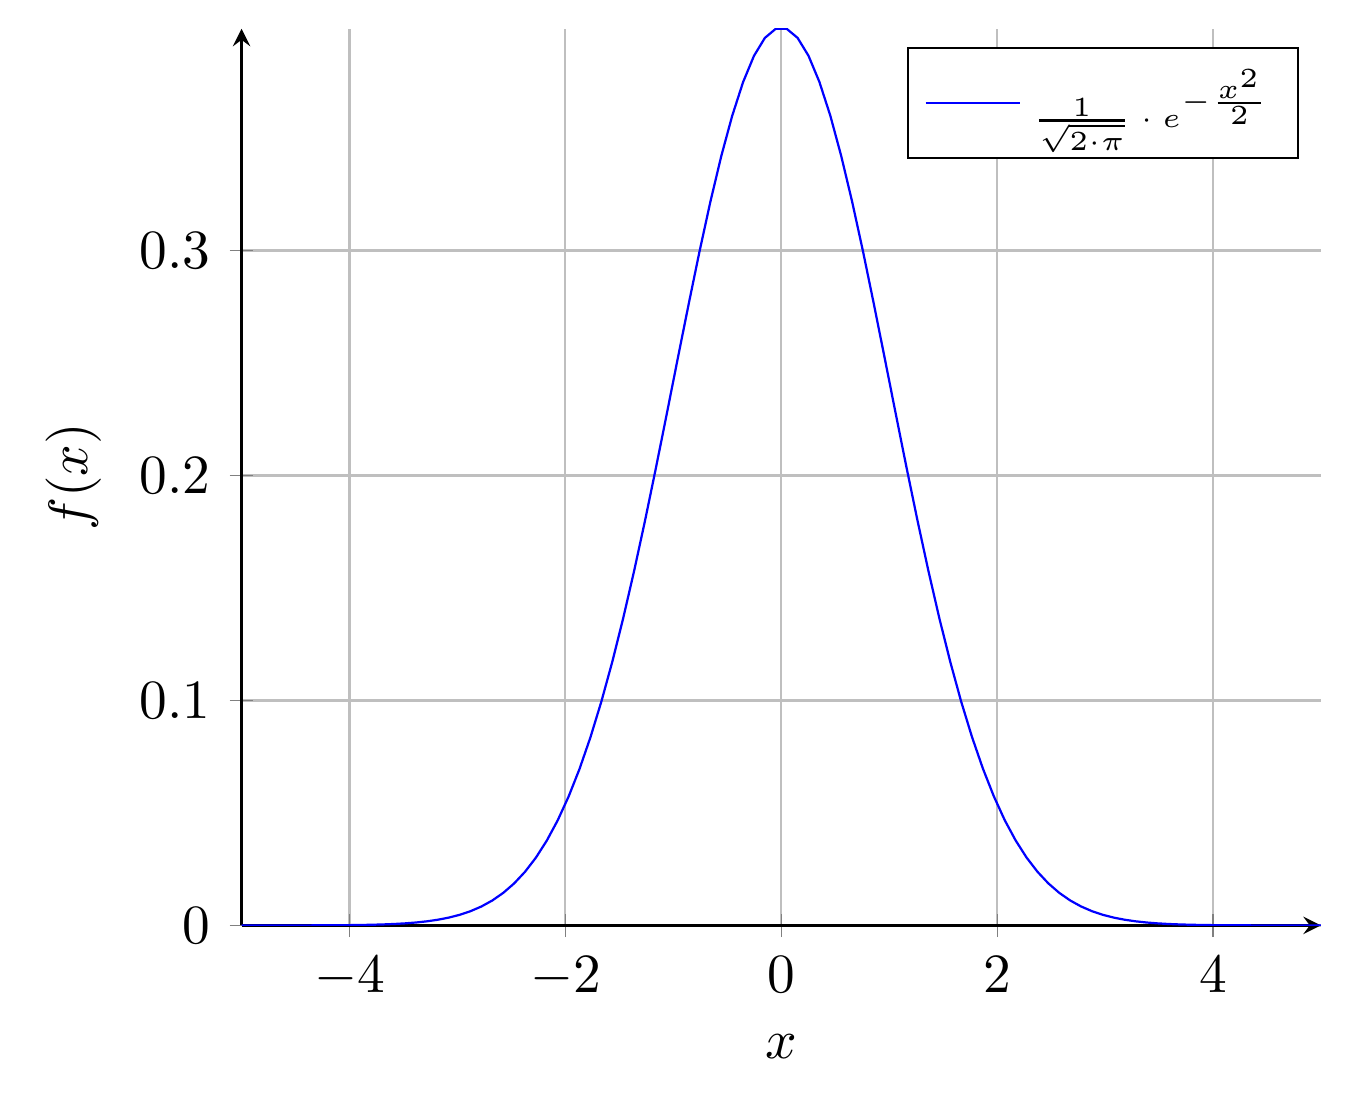
\begin{tikzpicture}[scale=2]
    \begin{axis}[
        axis lines = left,
        xlabel = \(x\),
        ylabel = {\(f(x)\)},
        ymajorgrids = true, 
        xmajorgrids = true,
    ]
    \addplot [
        domain=-5:5, 
        samples=100, 
        color=blue,
    ]
    {(1/sqrt(2*pi)) * e^(-x^2/2)};
    \addlegendentry{\tiny \(\frac{1}{\sqrt{2 \cdot \pi}} \cdot e^{-\frac{x^2}{2}}\)}
 
    \end{axis}
    \end{tikzpicture}    
\end{center}
